\subsection*{Appendix C}

In Table~\ref{tab:log-metrics}, I collect the out-of-sample performance metrics for each cutoff $X$ using the logistic model.

\begin{table}[H]
	\centering
	\begin{tabular}{||c c c c c||}
\hline
Days & AUC & Accuracy & Recall (1) & Recall (0) \\
\hline\hline
360 & 0.898 & 0.894 & 0.917 & 0.801 \\
240 & 0.890 & 0.865 & 0.868 & 0.858 \\
120 & 0.914 & 0.881 & 0.858 & 0.915 \\
60 & 0.932 & 0.896 & 0.866 & 0.934 \\
30 & 0.934 & 0.888 & 0.845 & 0.937 \\
14 & 0.933 & 0.895 & 0.859 & 0.936 \\
7 & 0.931 & 0.887 & 0.857 & 0.920 \\
1 & 0.942 & 0.899 & 0.859 & 0.943 \\
\hline
\end{tabular}

	\caption{Logistic Regression Performance by Cutoff}
	\label{tab:log-metrics}
\end{table}

In Figure~\ref{fig:log-roc}, I depict the area under the curve achieved by the MLE logistic regression for each cutoff.

\begin{figure}[H]
	\centering
	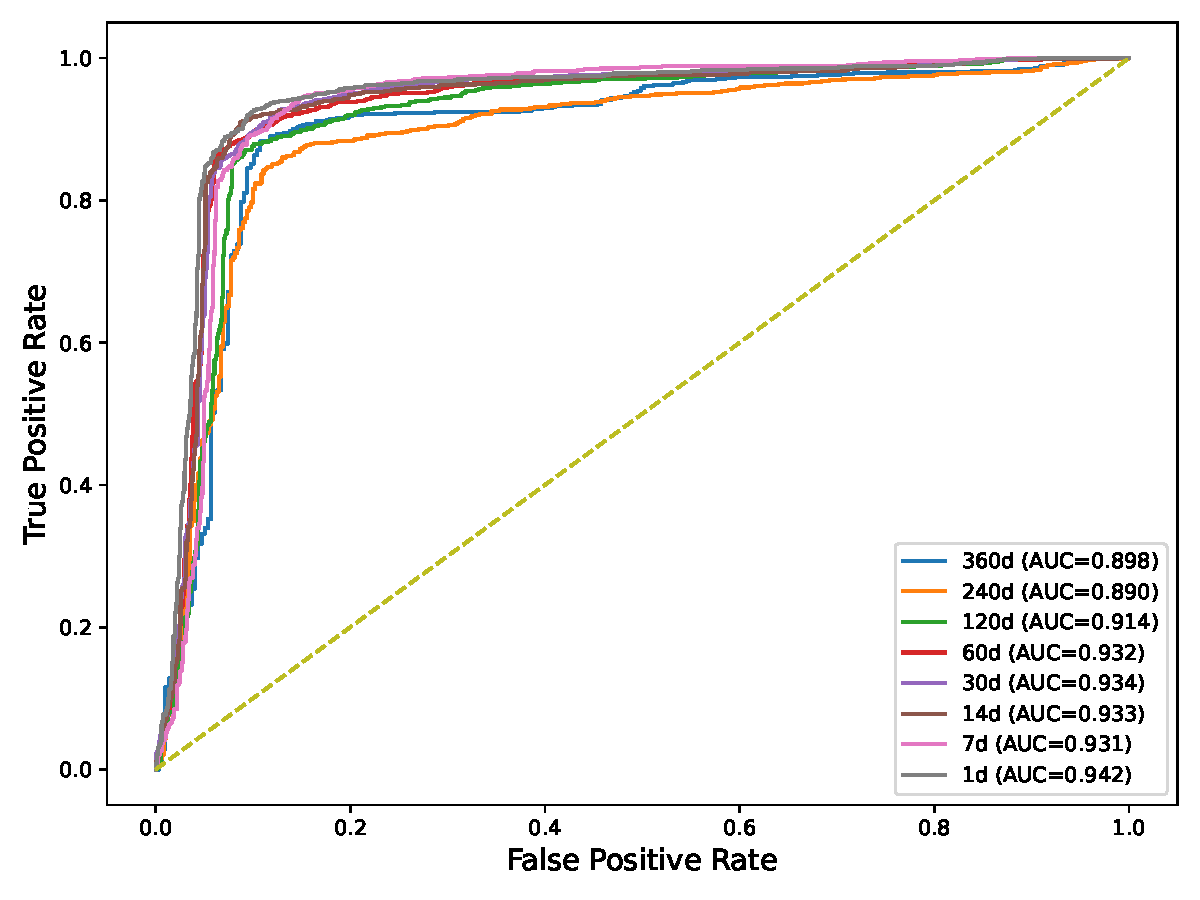
\includegraphics[width = 0.8\linewidth]{../Figures/log_roc.pdf}
	\caption{Logistic Models' AUCs}
	\label{fig:log-roc}
\end{figure}

Figure~\ref{fig:roi-beta}, similar to Figure~\ref{fig:roi-year}, simply depicts another way of examining the effect of campaign contributions on the probability of winning over time. 

\begin{figure}[H]
	\centering
	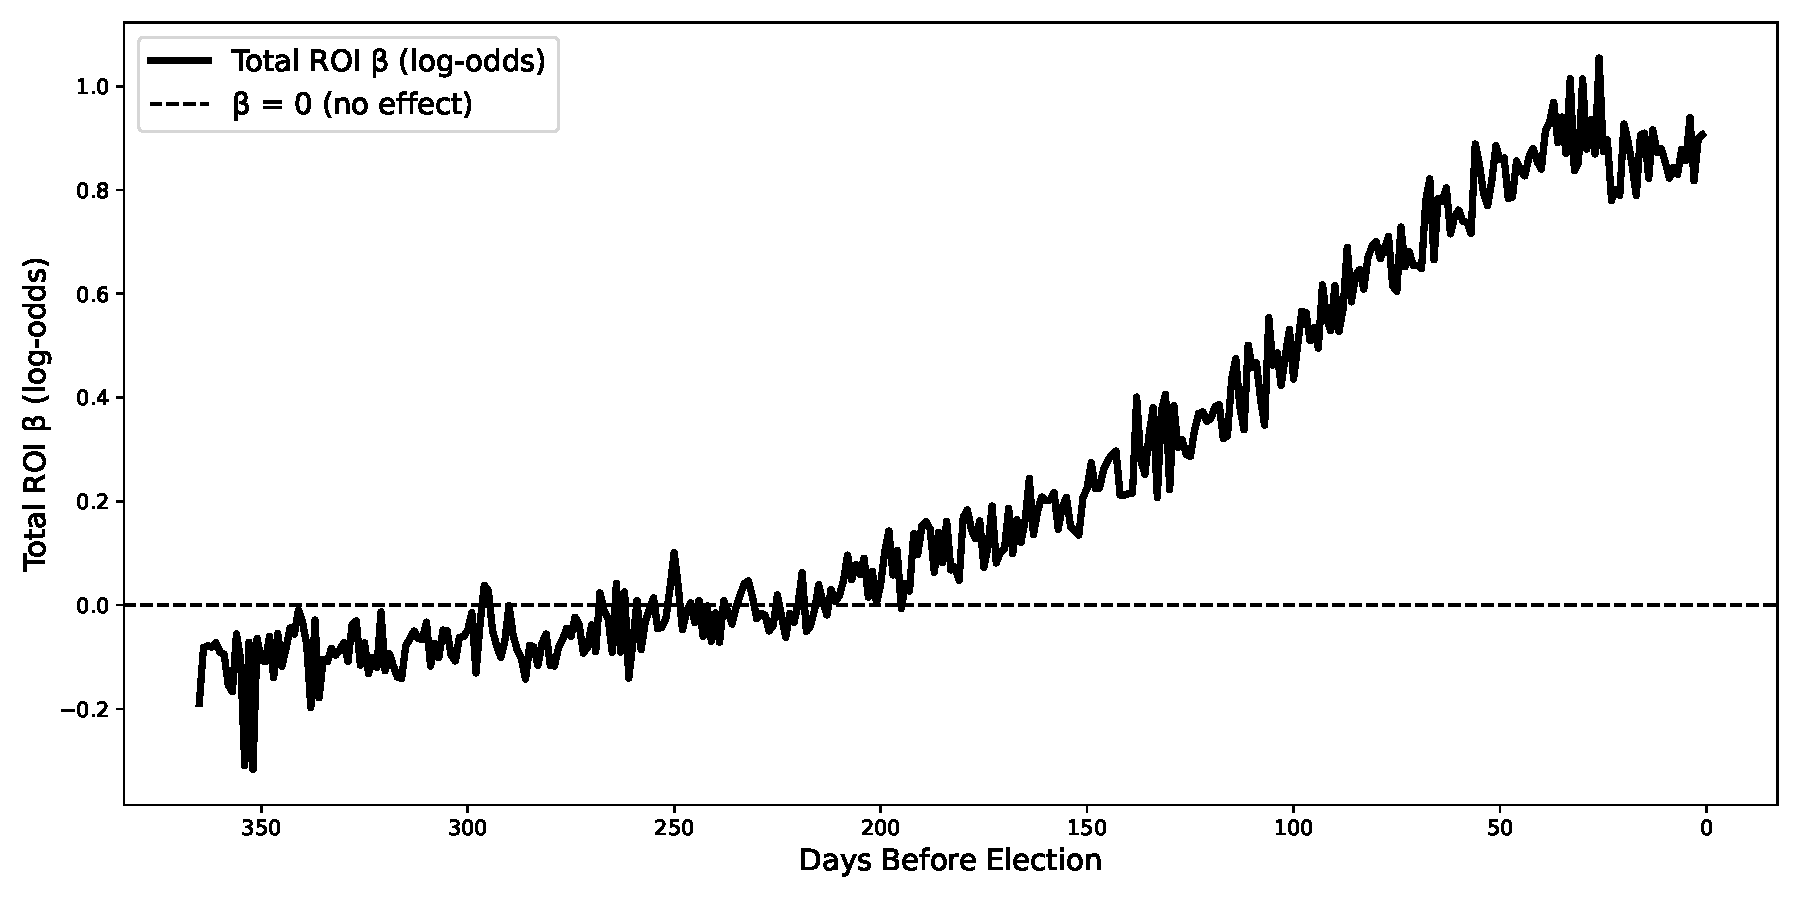
\includegraphics[width = 0.8\linewidth]{../Figures/roi_beta_over_time.pdf}
	\caption{Total (Raw) Return on Investment Trend a Year Prior to Election Day}
	\label{fig:roi-beta}
\end{figure}

Table~\ref{tab:gam-log-metrics} summarizes the GAM fits, showing AUC, accuracy, and recall for each cutoff.

\begin{table}[H]
	\centering
	\begin{tabular}{||c c c c c||}
\hline
Days & AUC & Accuracy & Recall (1) & Recall (0) \\
\hline\hline
360 & 0.914 & 0.896 & 0.939 & 0.724 \\
240 & 0.911 & 0.868 & 0.894 & 0.799 \\
120 & 0.938 & 0.887 & 0.891 & 0.882 \\
60 & 0.954 & 0.904 & 0.912 & 0.895 \\
30 & 0.960 & 0.904 & 0.909 & 0.898 \\
14 & 0.966 & 0.911 & 0.916 & 0.905 \\
7 & 0.963 & 0.909 & 0.928 & 0.887 \\
1 & 0.965 & 0.915 & 0.917 & 0.912 \\
\hline
\end{tabular}

	\caption{GAM Logistic Performance by Cutoff}
	\label{tab:gam-log-metrics}
\end{table}

Figure~\ref{fig:gam-or} depicts the odds-ratio trend over time using the logistic GAM.

\begin{figure}[H]
	\centering
	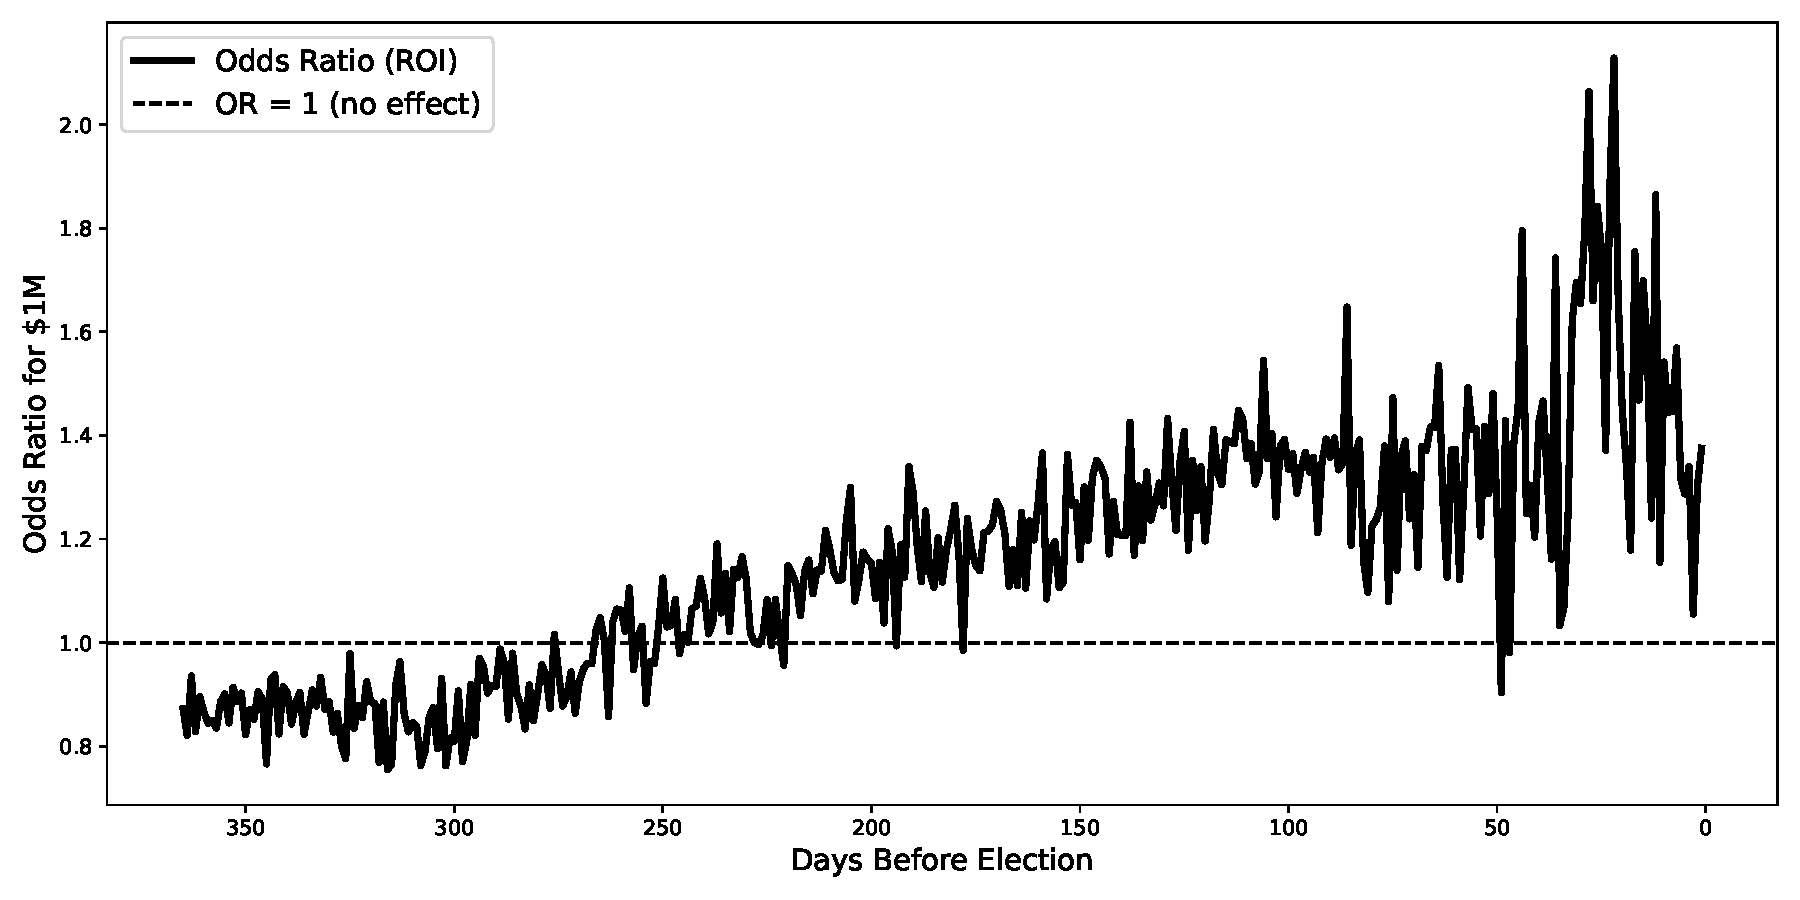
\includegraphics[width = 0.8\linewidth]{../Figures/gam_roi_over_time.pdf}
	\caption {GAM Total (Odds-Ratio) ROI Trend a Year Prior to Election Day}
	\label{fig:gam-or}
\end{figure}

Figure~\ref{fig:gam-roc} depicts the AUC achieved by the GAM logistic regression for each cutoff.

\begin{figure}[H]
	\centering
	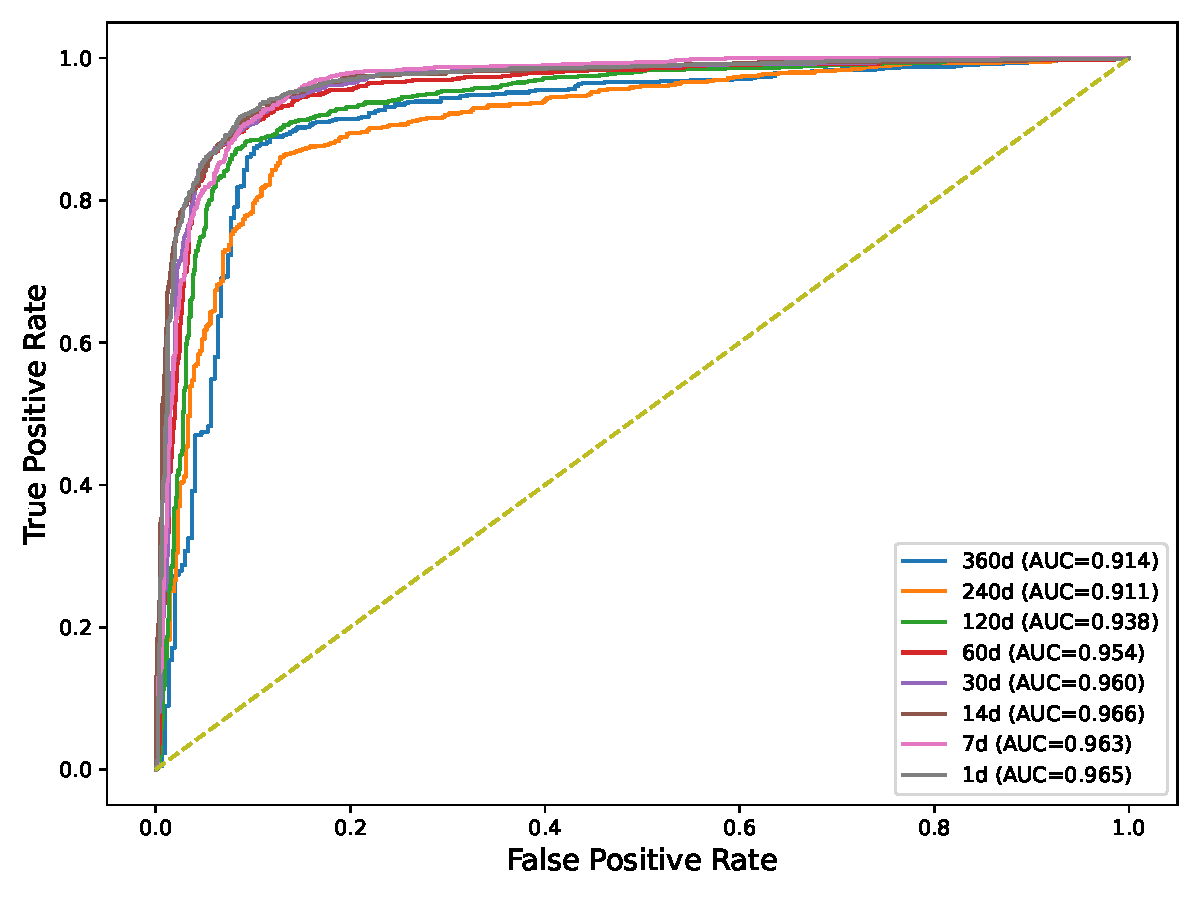
\includegraphics[width = 0.8\linewidth]{../Figures/gam_log_roc.pdf}
	\caption{Logistic GAM's AUCs}
	\label{fig:gam-roc}
\end{figure}

In Table~\ref{tab:ols-metrics}, I collect out-of-sample performance metrics ($R^2$, RMSE, MAE) and 5-fold CV $R^2$ for each cutoff from the simple least-squares models, while Table~\ref{tab:reg-r2} offers the regularized $R^2$ results and $\alpha$ given the better regularization technique (Ridge or LASSO).

\begin{table}[H]
	\centering
	\begin{minipage}{0.48\textwidth}
		\centering
		\begin{tabular}{||c c c c c||}
\hline
Days & $R^2$ & CV $R^2$ & RMSE & MAE \\
\hline\hline
360 & 0.410 & 0.393 & 13.672 & 9.715 \\
240 & 0.468 & 0.461 & 14.343 & 10.185 \\
120 & 0.555 & 0.560 & 14.372 & 10.208 \\
60 & 0.580 & 0.585 & 14.232 & 10.135 \\
30 & 0.587 & 0.596 & 14.168 & 9.980 \\
14 & 0.603 & 0.599 & 13.899 & 9.837 \\
7 & 0.609 & 0.601 & 13.926 & 9.987 \\
1 & 0.595 & 0.601 & 14.163 & 10.157 \\
\hline
\end{tabular}

		\caption{Least-Squares Regression Performance by Cutoff}
		\label{tab:ols-metrics}
	\end{minipage}\hfill
	\begin{minipage}{0.48\textwidth}
		\centering
		\begin{tabular}{||c c c||}
\hline
Days & Best Model ($\alpha$) & $R^2$ \\
\hline\hline
360 & RidgeCV (100.0000) & 0.410 \\
240 & RidgeCV (100.0000) & 0.468 \\
120 & LassoCV (0.1000) & 0.556 \\
60 & RidgeCV (17.7828) & 0.580 \\
30 & LassoCV (0.0316) & 0.588 \\
14 & LassoCV (0.0562) & 0.604 \\
7 & RidgeCV (31.6228) & 0.609 \\
1 & LassoCV (0.0562) & 0.595 \\
\hline
\end{tabular}

		\caption{Regularized $R^2$ for Each Cutoff}
		\label{tab:reg-r2}
	\end{minipage}
\end{table}

Table~\ref{tab:ho-metrics} reveals the hold-out performance for the linear GAM models.

\begin{table}[H]
	\centering
	\begin{tabular}{||c c c c||}
\hline
Days & HO $R^2$ & HO RMSE & HO MAE \\
\hline\hline
360 & 0.515 & 12.397 & 8.219 \\
240 & 0.532 & 13.452 & 9.051 \\
120 & 0.140 & 19.982 & 9.695 \\
60 & 0.522 & 15.178 & 9.454 \\
30 & 0.655 & 12.945 & 8.888 \\
14 & 0.695 & 12.180 & 8.583 \\
7 & 0.690 & 12.396 & 8.631 \\
1 & 0.693 & 12.322 & 8.728 \\
\hline
\end{tabular}

	\caption{GAM Linear Hold-Out Performance by Cutoff}
	\label{tab:ho-metrics}
\end{table}

Finally, the ROI of campaign contributions might also be expressed as elasticities, a unit-free measure of responsiveness. Raw elasticities measure the percent change in the probability of winning from a one percent increase in campaign contributions at a particular cutoff. Although not demonstrated here (due to the fact that I did not calculate the elasticities for each day across an entire election cycle), total spending over a political campaign may be thought of as a dynamic control/budget constraint problem. If total spending over the campaign is allocated across discrete time windows, it is natural that the sum of those period elasticities equal $1$: a one percent reallocation of total spending among time periods changes total spending by zero, so it cannot change the outcome in first order. Should anyone desire to calculate the ROI over an entire election cycle, this should be the result. 

For the sake of my goals, I calculated the raw elasticities for the arbitrary cutoffs I used throughout my research, as well as for the win-probability models across an entire year of campaigning. Because they are independent snapshots, they will \textit{not} sum to one; these elasticities are partial derivatives at particular time windows, so we do not get a partition of ``total elasticity.'' Furthermore, normalized elasticities tell one the share of total responsiveness that comes from spending at time $X$ (of the entire effect budget, what fraction is due to period $X$?). I also implemented these calculations, allowing one to compare periods directly on a common scale, leaving only the relative pattern over time. Altogether, this gives one another way to understand the ROI of campaign contributions.

\begin{table}[H]
	\centering
	\begin{minipage}{0.48\textwidth}
		\centering
		\begin{tabular}{||c c||}
\hline
Days & Elasticity \\
\hline\hline
360 & -0.012 \\
240 & -0.006 \\
120 & 0.177 \\
60 & 0.581 \\
30 & 1.129 \\
14 & 1.738 \\
7 & 1.683 \\
1 & 1.707 \\
\hline
\end{tabular}

		\caption{Raw Elasticities for MLE Logistic}
		\label{tab:log-elast}
	\end{minipage}\hfill
	\begin{minipage}{0.48\textwidth}
		\centering
		\begin{tabular}{||c c||}
\hline
Days & Elasticity \\
\hline\hline
360 & -0.029 \\
240 & 0.012 \\
120 & 0.084 \\
60 & -0.069 \\
30 & 0.370 \\
14 & 0.040 \\
7 & 0.406 \\
1 & 0.197 \\
\hline
\end{tabular}

		\caption{Raw Elasticities for GAM Logistic}
		\label{tab:log-gam-elast}
	\end{minipage}
\end{table}

\begin{table}[H]
	\centering
	\begin{minipage}{0.48\textwidth}
		\centering
		

		\caption{Raw Elasticities for Linear}
		\label{tab:lin-elast}
	\end{minipage}\hfill
	\begin{minipage}{0.48\textwidth}
		\centering
		\begin{tabular}{||c c||}
\hline
Days & Elasticity \\
\hline\hline
360 & -0.002 \\
240 & -0.001 \\
120 & 0.010 \\
60 & 0.020 \\
30 & 0.015 \\
14 & -0.004 \\
7 & -0.007 \\
1 & -0.006 \\
\hline
\end{tabular}

		\caption{Raw Elasticities for GAM Linear}
		\label{tab:lin-gam-elast}
	\end{minipage}
\end{table}

\begin{figure}[H]
	\centering
	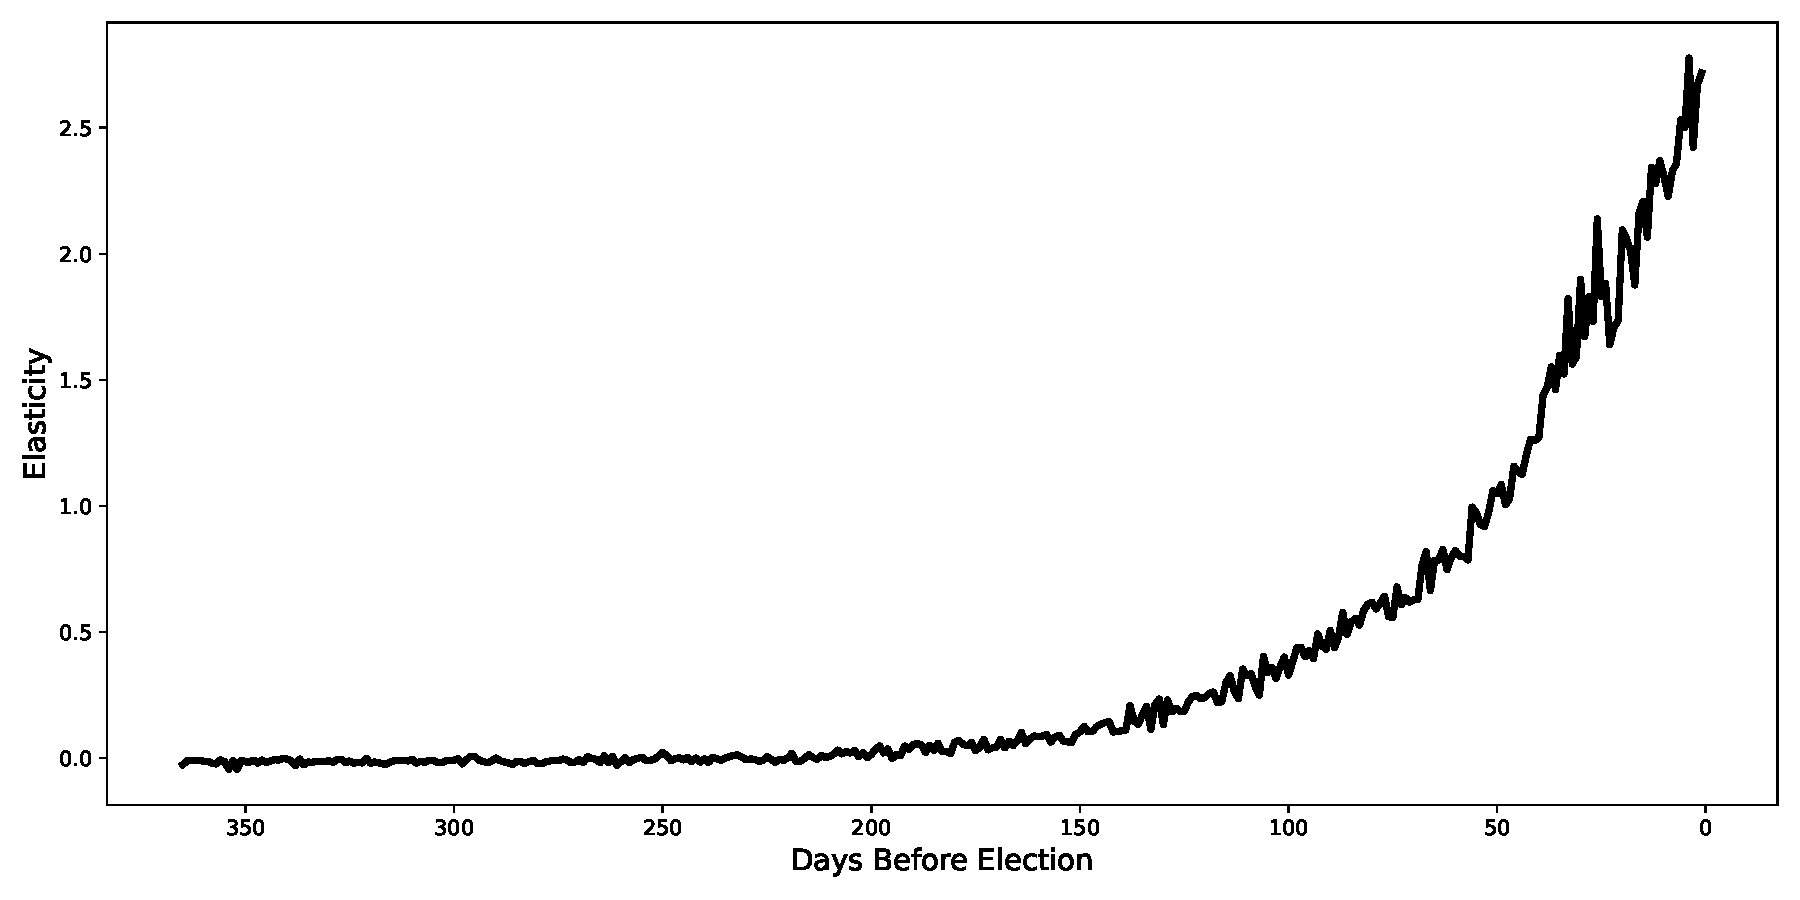
\includegraphics[width=0.8\linewidth]{../Figures/elasticity_over_time.pdf}
	\caption{MLE Logistic Model's Raw Elasticities over Time}
	\label{fig:log-e-time}
\end{figure}

\begin{figure}[H]
	\centering
	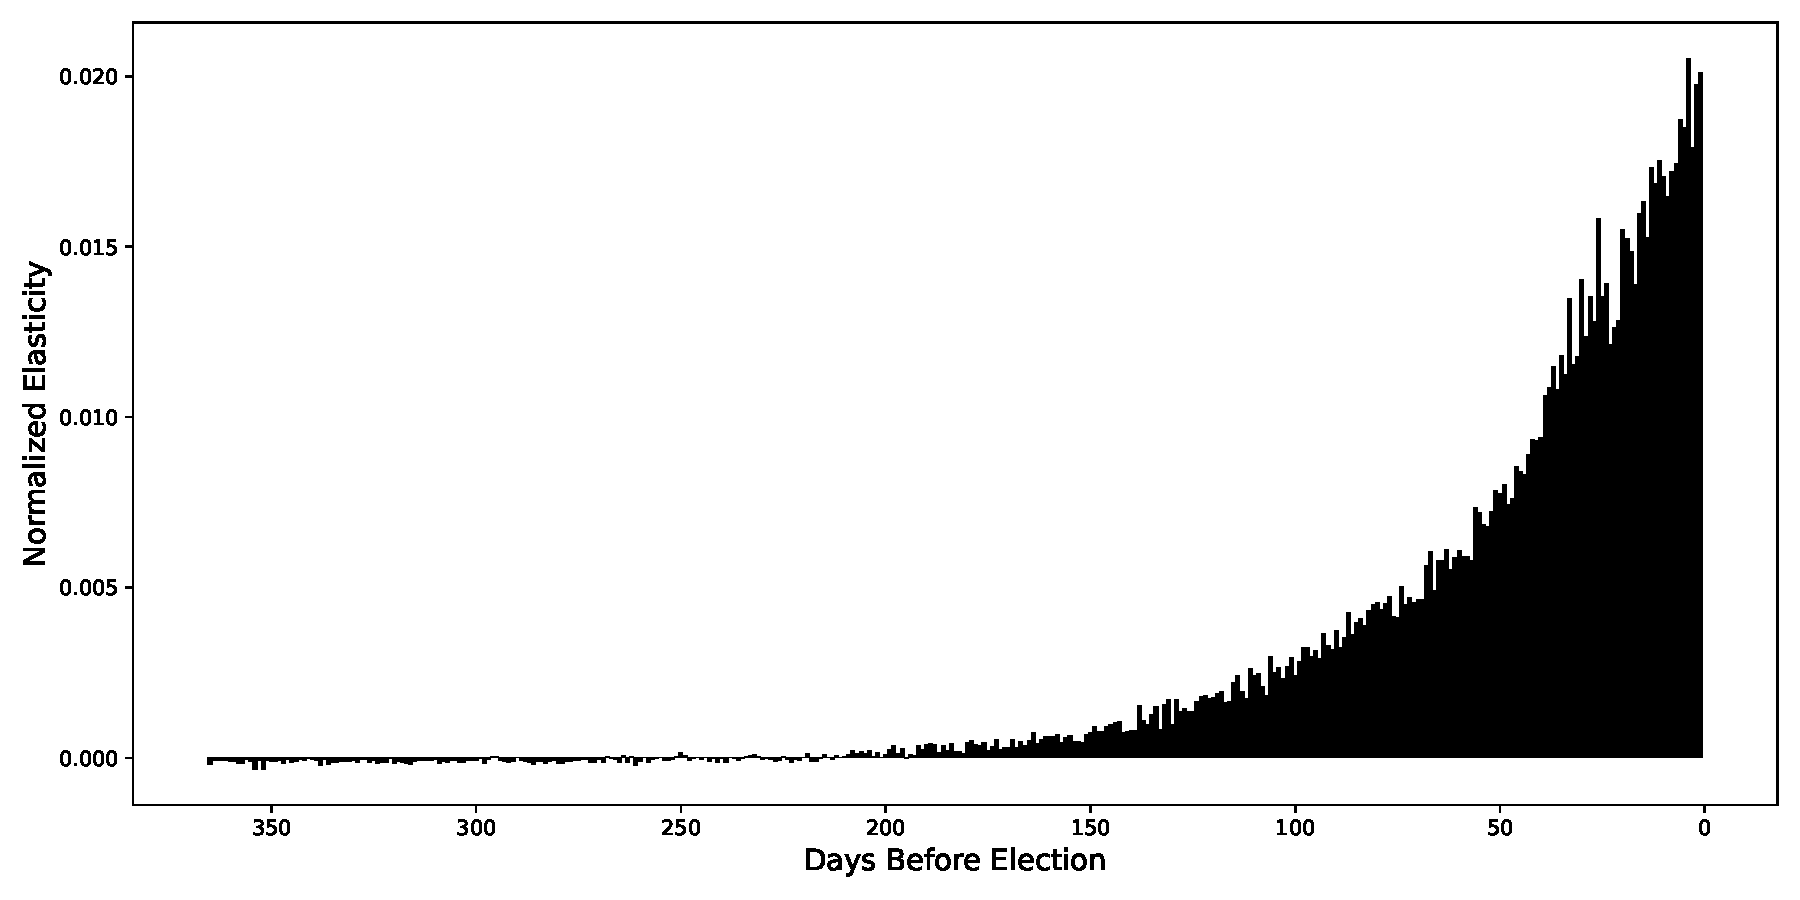
\includegraphics[width=0.8\linewidth]{../Figures/norm_elast_over_time.pdf}
	\caption{MLE Logistic Model's Normalized Elasticities over Time}
	\label{fig:log-norm-e-time}
\end{figure}

\begin{figure}[H]
	\centering
	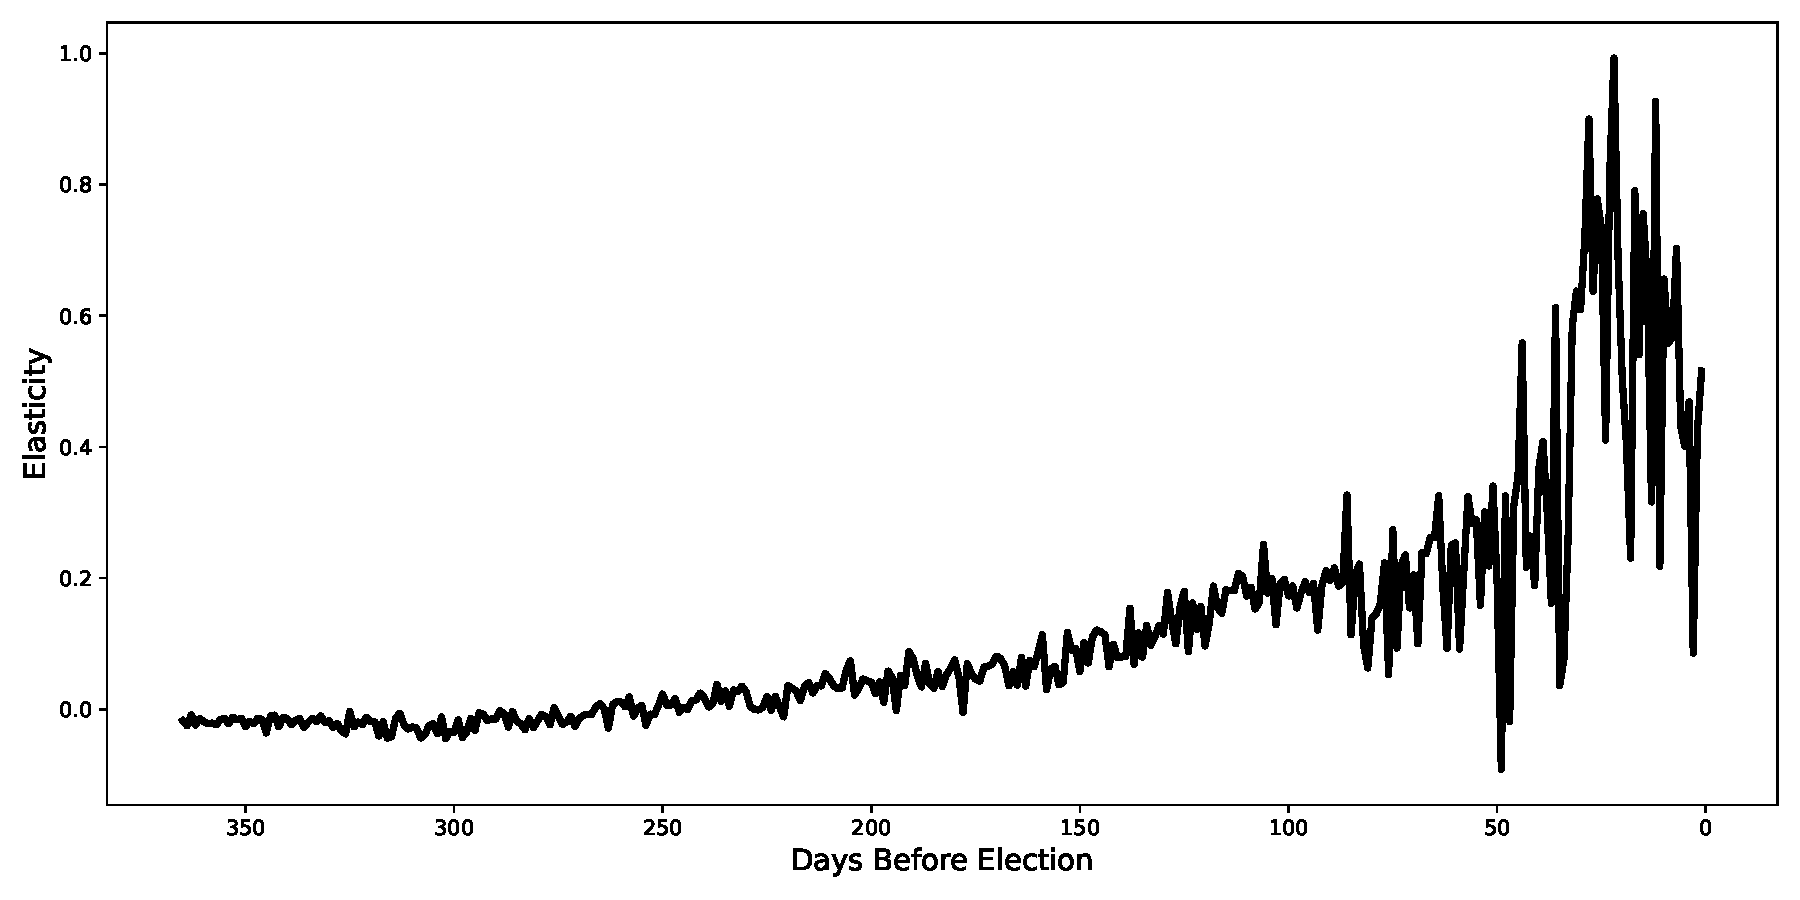
\includegraphics[width=0.8\linewidth]{../Figures/gam_elasticity_over_time.pdf}
	\caption{Logistic GAM's Raw Elasticities over Time}
	\label{fig:gam-log-e-time}
\end{figure}

\begin{figure}[H]
	\centering
	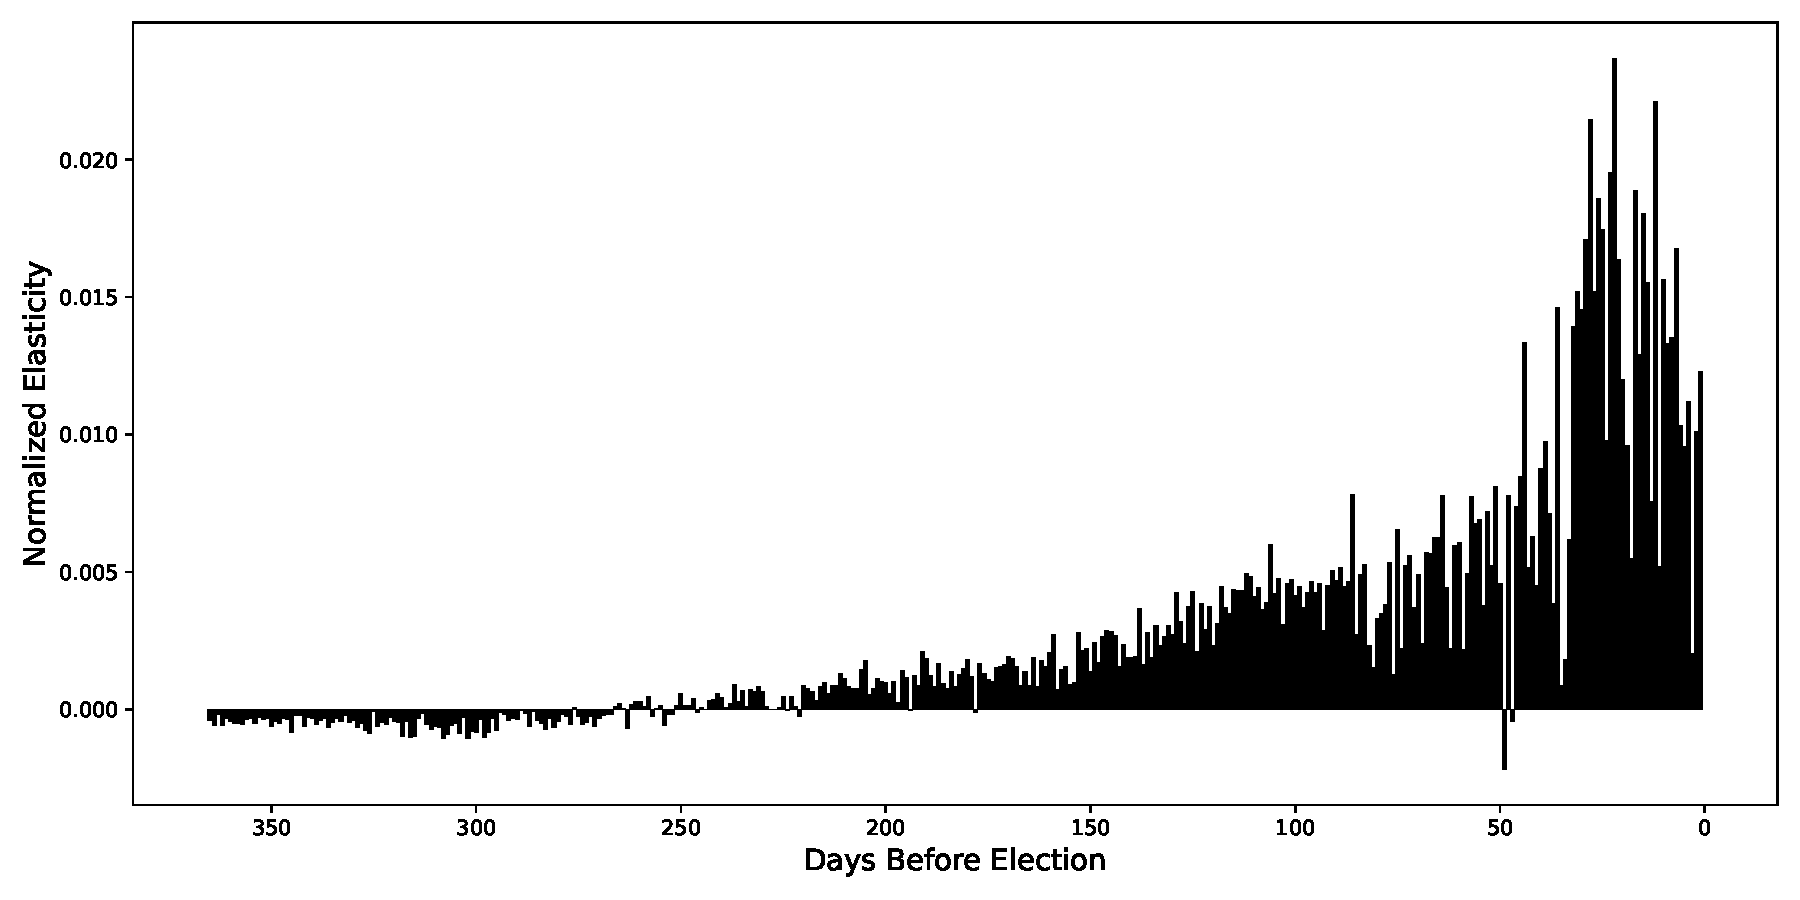
\includegraphics[width=0.8\linewidth]{../Figures/gam_norm_elast_over_time.pdf}
	\caption{Logistic GAM's Normalized Elasticities over Time}
	\label{fig:gam-log-norm-e-time}
\end{figure}



\newpage
